\label{sec:introduction}

In wood industry, finished products are typically obtained through machining processes in which a semi-finished component, such as a wood panel, is processed using a machine known as a \emph{work center}, shown in Fig.~\ref{fig:worktable}.

A typical work center is equipped with a tool storage system from which the tools required to perform operations such as cutting, milling, and contouring on the panel are automatically selected. However, the use of these tools can induce vibrations and oscillations in the workpiece, thereby reducing the quality of the final product~\cite{trappey1990literature,jackson2002waves}. For this reason, keeping the workpiece as stable and firm as possible during machining is crucial.

The work center is equipped with a worktable featuring movable bars that translate along the machine’s horizontal axis, above which vacuum suction cup fixtures can be positioned.

The fixtures can be square or rectangular in shape (Fig.~\ref{fig:suction_cups}) and are composed of a square base, which allows them to be mounted on the bars and to slide along their length. To improve product quality through an appropriate fixture layout, the fixtures can also be freely rotated to achieve better alignment with the shape of the workpiece.

\begin{figure}[t]
	\centering
	\begin{subfigure}[b]{0.3\textwidth}
		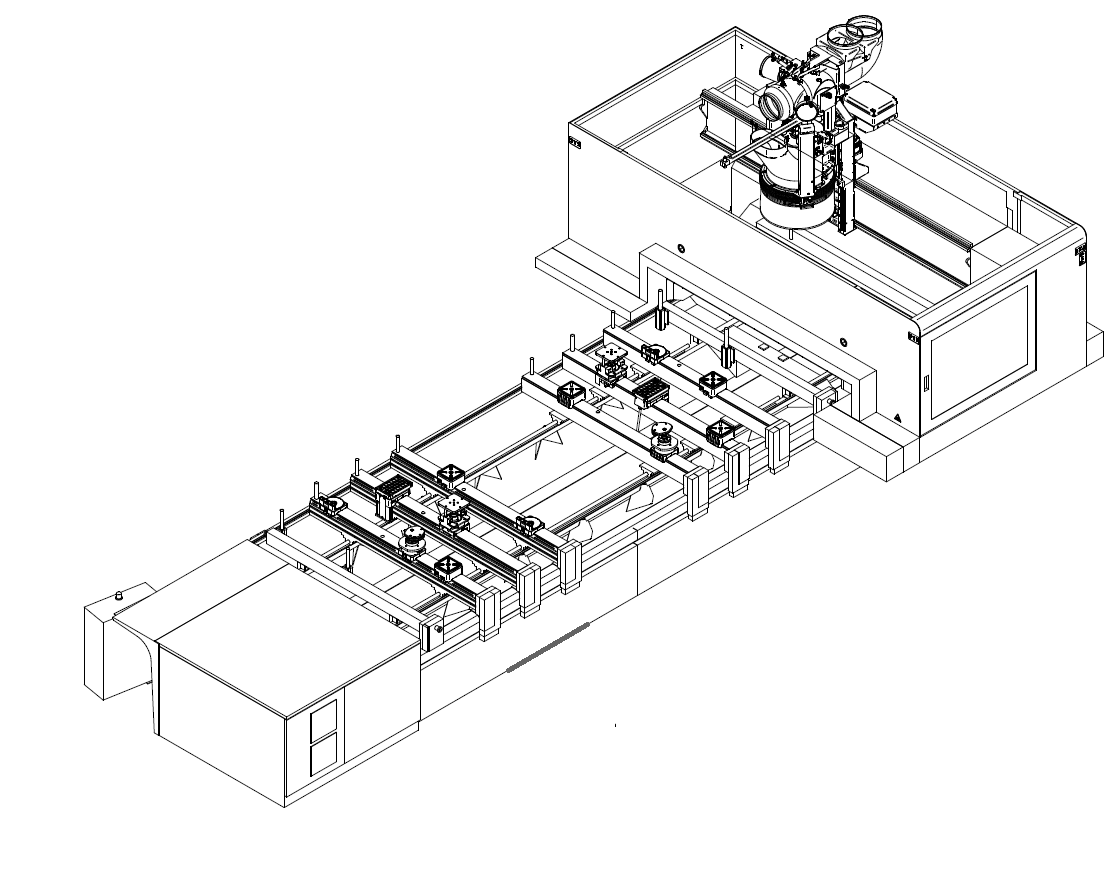
\includegraphics[width=\textwidth]{img/worktable.png}
		\caption{Work center}
		\label{fig:worktable}
	\end{subfigure}
	\hspace{2cm}
	\begin{subfigure}[b]{0.3\textwidth}
		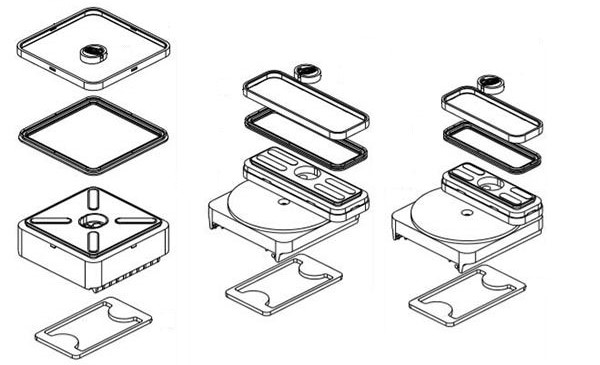
\includegraphics[width=\textwidth]{img/suction_cups_schema_no_dimnesion.jpg}
		\caption{Vacuum suction cup fixtures}
		\label{fig:suction_cups}
	\end{subfigure}
	\caption{On the left, a work center featuring a worktable with movable bars. On the right, fixtures used to secure the workpiece during machining operations.}
	\label{fig:problem_description_img}
\end{figure}


Determining an appropriate fixture layout for a given workpiece is not always straightforward for a human operator, especially when the workpiece has contoured shapes or includes areas to be extruded. Layouts are often based on the operator’s experience; however, such manually designed solutions are not necessarily optimal and can often be improved by considering the structural properties of the fixtures system, such as its resistance to bending and torsional forces.

In this paper, we aim to determine a sound and possibly optimal placement of fixtures beneath the workpiece by identifying, the type, position, and rotation angle of the fixtures that can be used to sustain it. Our approach consists of two stages. First, we compute a feasible, but generally sub-optimal, placement by solving a simplified version of the original problem in which fixture rotations are neglected. To this end, we compare the quality of the solutions obtained using a Constraint Programming (CP) solver and a Reinforcement Learning (RL) algorithm. Second, the resulting layouts are refined through a local search procedure based on Particle Swarm Optimization (PSO), which explicitly accounts for fixture rotations.

This work extends~\cite{vitali2026constraint}, which proposed a hybrid approach combining Constraint Programming (CP), Mixed Integer Programming (MIP), and Particle Swarm Optimization (PSO) to solve the fixture layout optimization problem.  We reformulated several constraints of the CP model, improving its performance on the most challenging instances for the considered solvers, and extend the experimental evaluation by introducing additional real-world case studies. Additionally, we propose a Q-learning-based algorithm for solving the simplified version of the problem and compare its performance with those of the CP and MIP models.

Experimental results show that the solutions produced by the CP and MIP models are of higher quality than those obtained using Q-learning and consistently outperform those designed by an expert operator. Starting from any of these initial layouts, PSO further improves the solution by increasing the moments of inertia of the fixture configuration, thereby enhancing workpiece stability.\footnote{This work was carried out in collaboration with a leading company in the woodworking machinery sector. The name of the company is omitted for privacy reasons.}

\emph{Paper structure.} The paper is organized as follows. Section~\ref{sec:related_work} reviews the related work. Section~\ref{sec:backgorund} presents the background context.  Section~\ref{sec:problem_description} describes the problem parameters and constraints. Section~\ref{sec:cp_model} introduces the CP model, while Section~\ref{sec:mip_model} presents the MIP model. Section~\ref{sec:rl_algorithm} introduces the Q-learning based algorithm. Section~\ref{sec:pso_algorithm} describes the PSO-based algorithm. Finally, Section~\ref{sec:result_analysis} discusses the experimental results, and Section~\ref{sec:conclusions} concludes the paper.